\subsubsection{example}
The obtained results were the following:
{
\renewcommand{\arraystretch}{2}
\begin{longtable}[h]{| c | c | c | c | c |}
    \hline
    \textbf{Failures} & \multicolumn{3}{c}{Time limit} & \\
    \hline
    \textbf{Search strategy} & \textbf{\textit{30 sec}} & \textbf{\textit{1 min}} & \textbf{\textit{2 min}} & \textbf{\textit{5 min}} \\
    \hline
    \endhead
    default search                                &    353 &     353 &     353 &      353 \\
    \hline
    \textit{domWdeg, random}                      &    345 &     345 &     345 &      345 \\
    \hline
    domWdeg, random, Luby restart L=250           &   2.936 &    2.936 &    2.936 &     2.936 \\
    \hline
    domWdeg, random, Luby restart L=250, LNS 85\% &  13.902 &   28.127 &   57.279 &   152.811 \\
    \hline
    domWdeg, random, Luby restart L=250, LNS 15\% & 989.744 & 1.915.201 & 3.993.931 & 10.631.389 \\
    \hline
    first fail, min                               &    687 &     687 &     687 &      687 \\
    \hline
\end{longtable}
}
\begin{figure}[H]
    \centering
    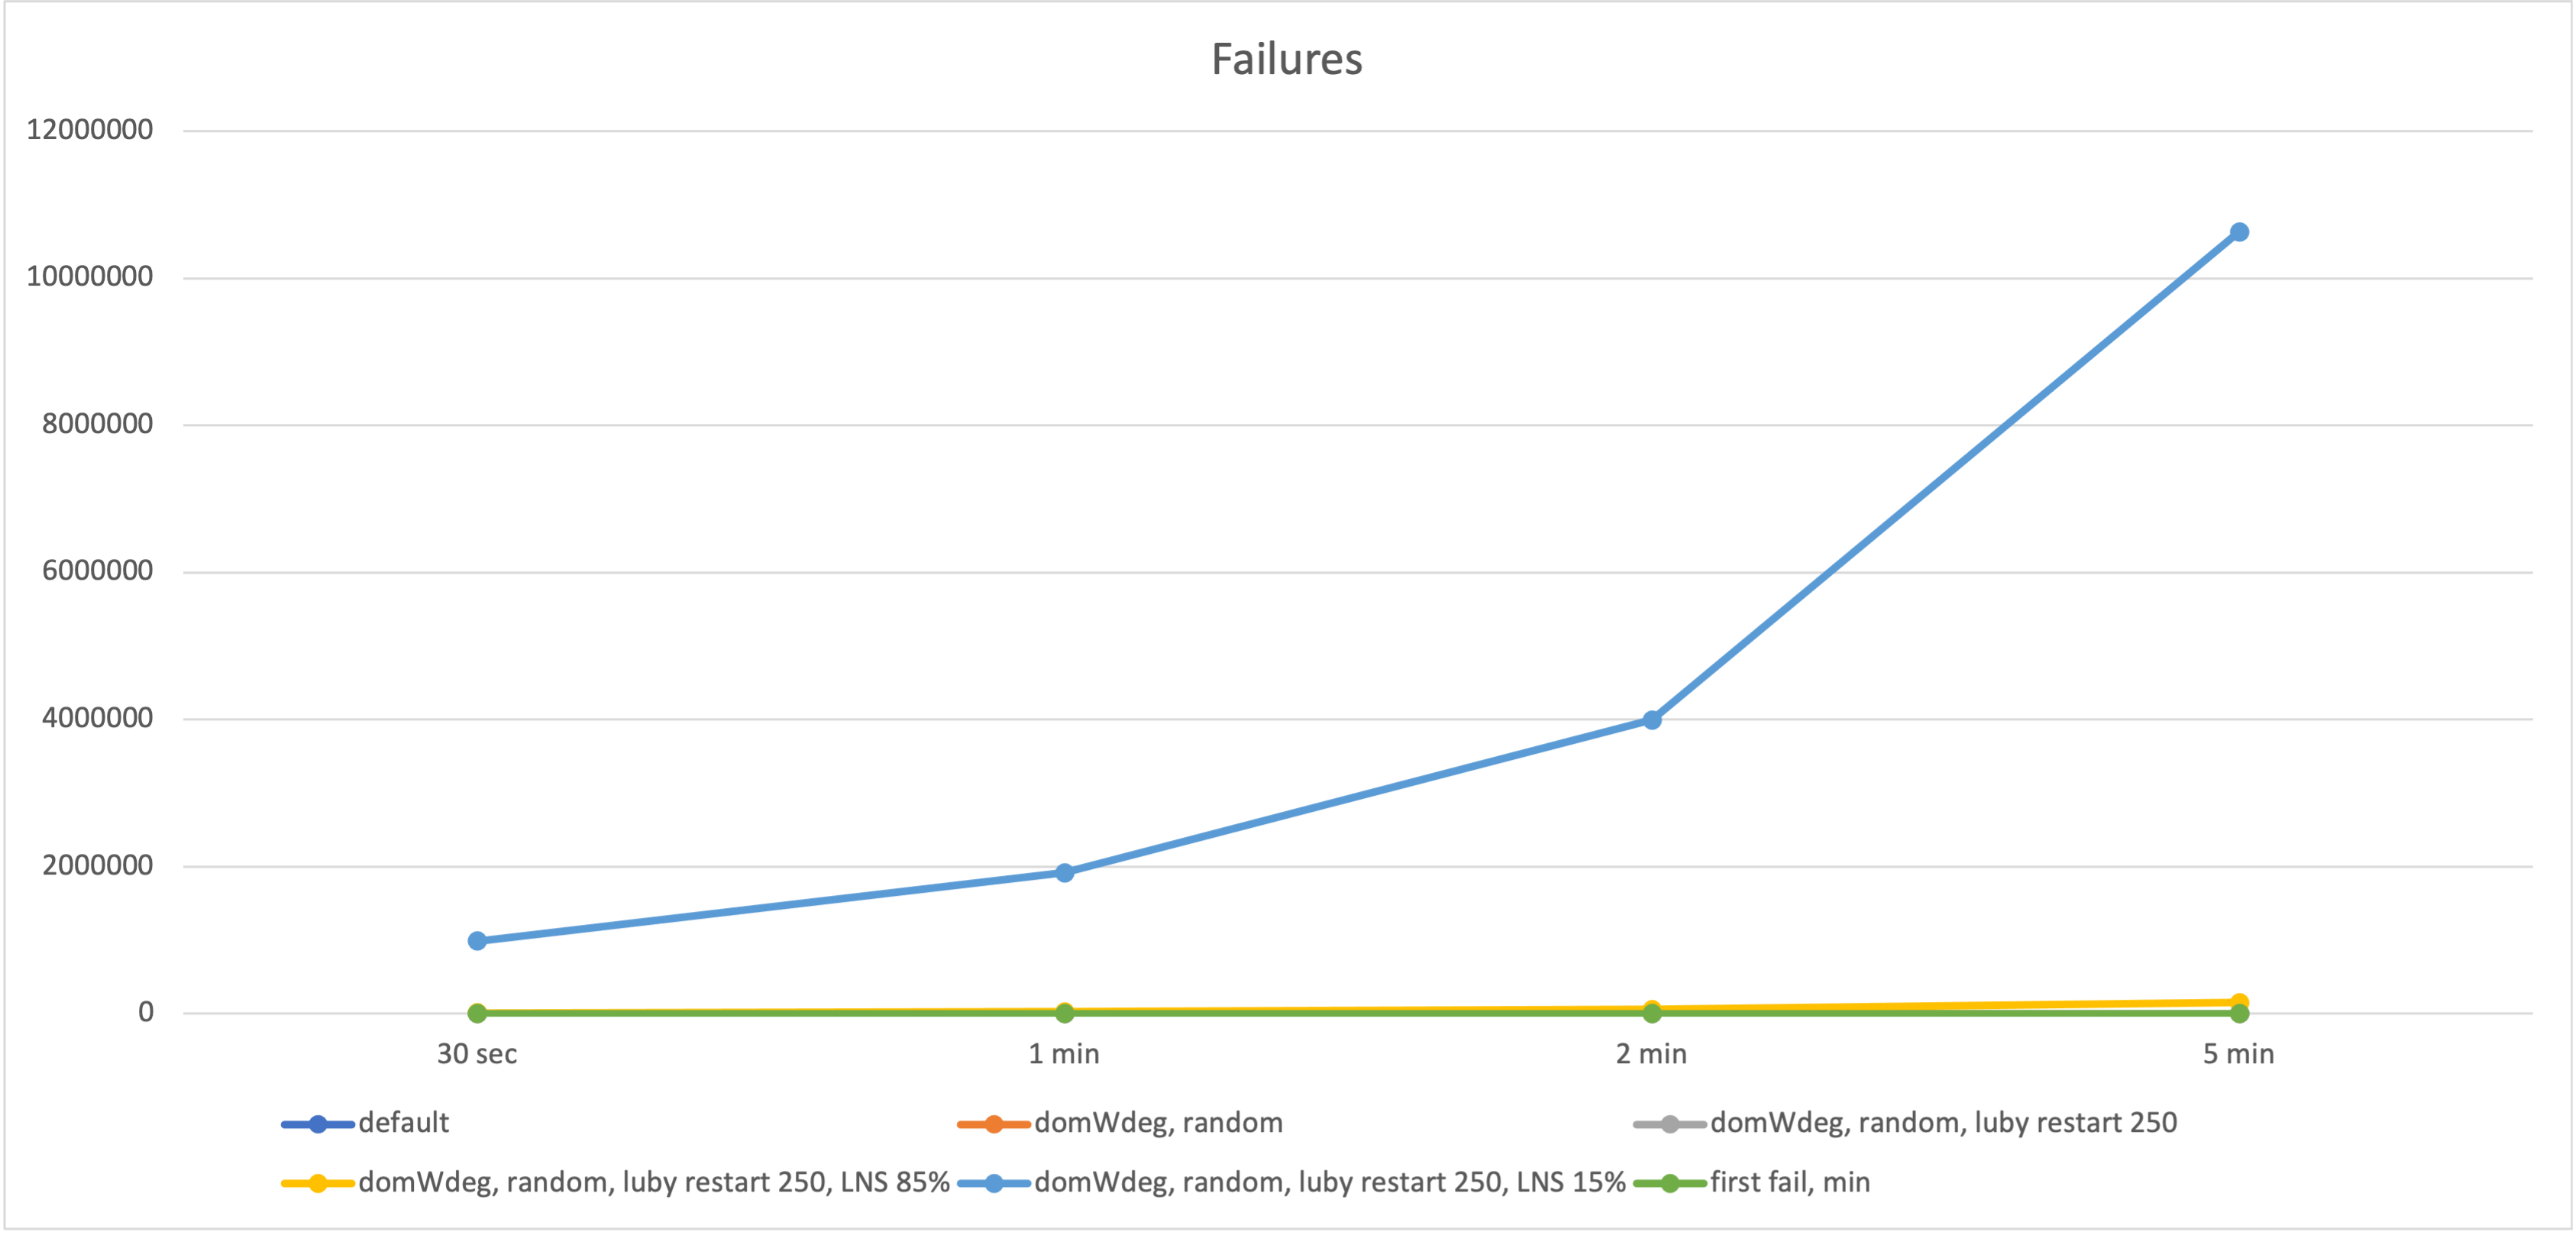
\includegraphics[width=1.0\columnwidth]{../graphs/example-failures.png}
    \caption{Failures graph for example.}
\end{figure}

{
\renewcommand{\arraystretch}{2}
\begin{longtable}[h]{| c | c | c | c | c |}
    \hline
    \textbf{Objective function} & \multicolumn{3}{c}{Time limit} & \\
    \hline
    \textbf{Search strategy} & \textbf{\textit{30 sec}} & \textbf{\textit{1 min}} & \textbf{\textit{2 min}} & \textbf{\textit{5 min}} \\
    \hline
    \endhead
    default search                                & 496.120 & 496.120 & 496.120 & 496.120 \\
    \hline
    \textit{domWdeg, random}                      & 496.120 & 496.120 & 496.120 & 496.120 \\
    \hline
    domWdeg, random, Luby restart L=250           & 496.120 & 496.120 & 496.120 & 496.120 \\
    \hline
    domWdeg, random, Luby restart L=250, LNS 85\% & 533.690 & 533.690 & 533.690 & 533.690 \\
    \hline
    domWdeg, random, Luby restart L=250, LNS 15\% & 496.120 & 496.120 & 496.120 & 496.120 \\
    \hline
    first fail, min                               & 496.120 & 496.120 & 496.120 & 496.120 \\
    \hline
\end{longtable}
}

\begin{figure}[H]
    \centering
    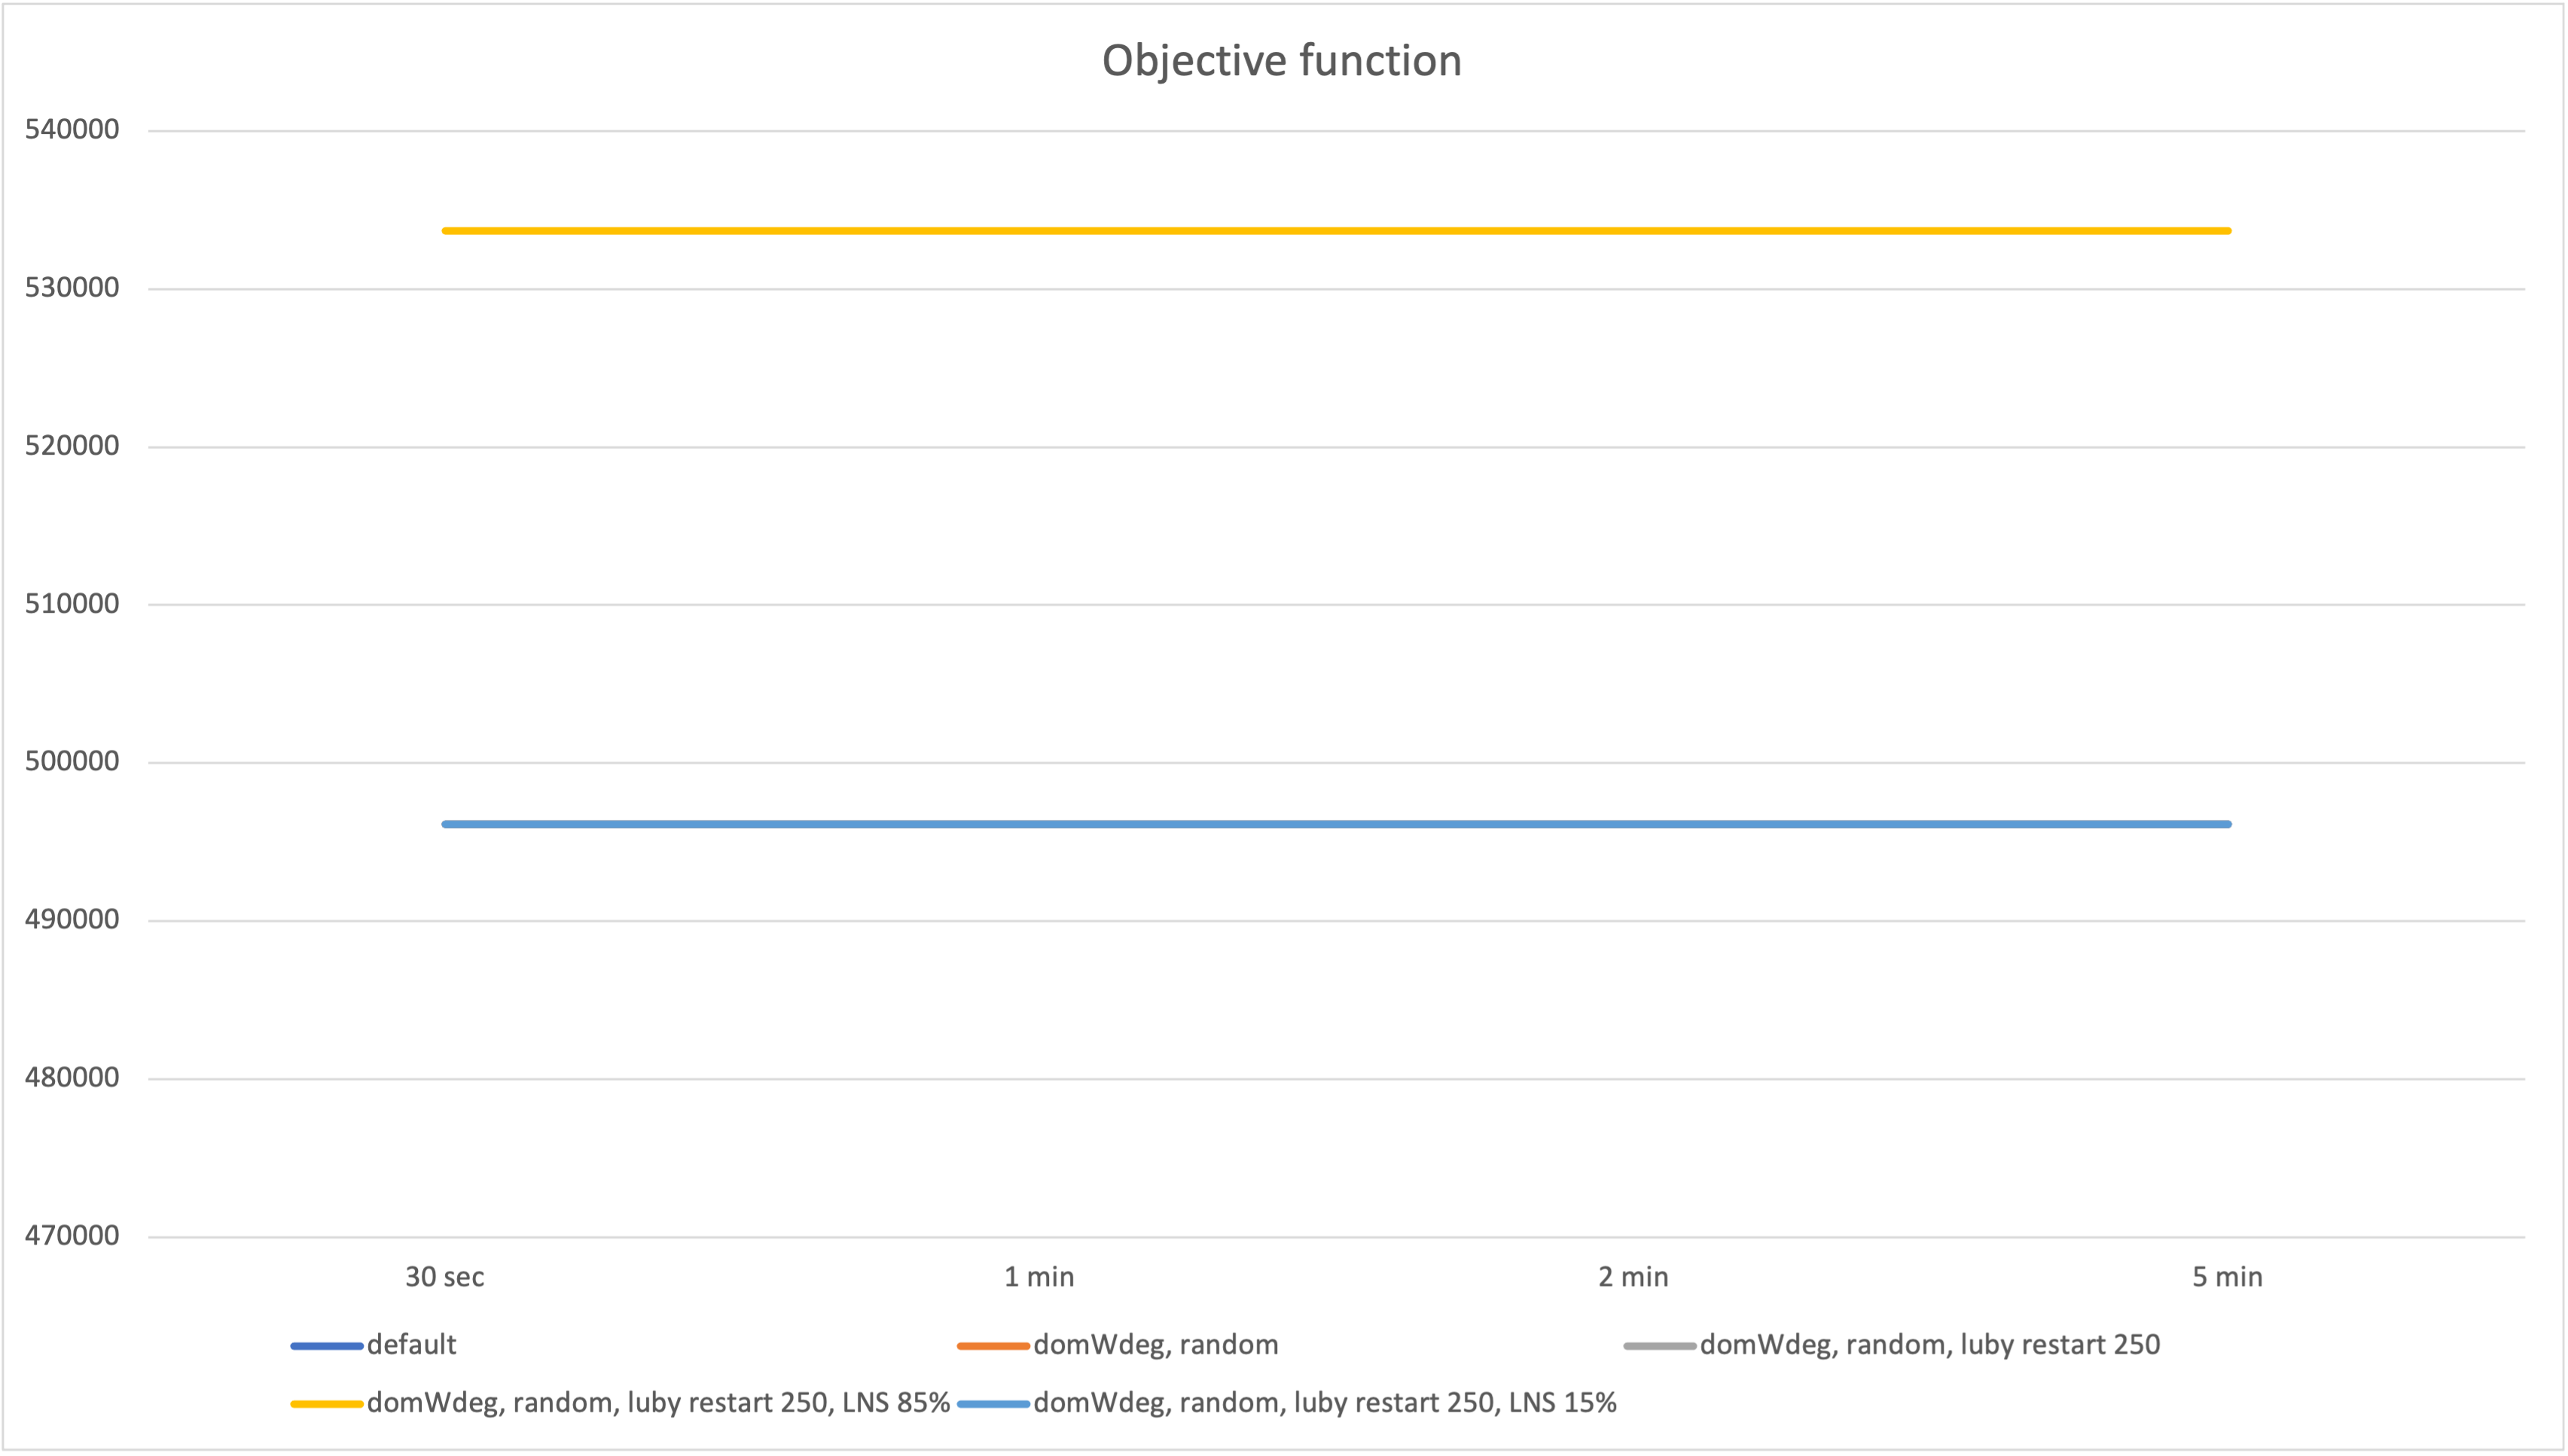
\includegraphics[width=1.0\columnwidth]{../graphs/example-objf.png}
    \caption{Objective functions graph for example.}
\end{figure}

{
\renewcommand{\arraystretch}{2}
\begin{longtable}[h]{| c | c | c | c |}
    \hline
    \textbf{Weights} & \textbf{Objective function} & \textbf{Total distance} & \textbf{Used vehicles} \\
    \hline
    \endhead
    $\alpha = 10, \beta = 0$ & 496.120 & 49.612 & 2 \\
    \hline
    $\alpha = 7, \beta = 3$  & 347.293 & 49.612 & 3 \\
    \hline
    $\alpha = 5, \beta = 5$  & 248.075 & 49.612 & 3 \\
    \hline
    $\alpha = 3, \beta = 7$  & 148.857 & 49.612 & 3 \\
    \hline
    $\alpha = 0, \beta = 10$ &      30 & 63.012 & 3 \\
    \hline
\end{longtable}
}

\begin{figure}[H]
    \centering
    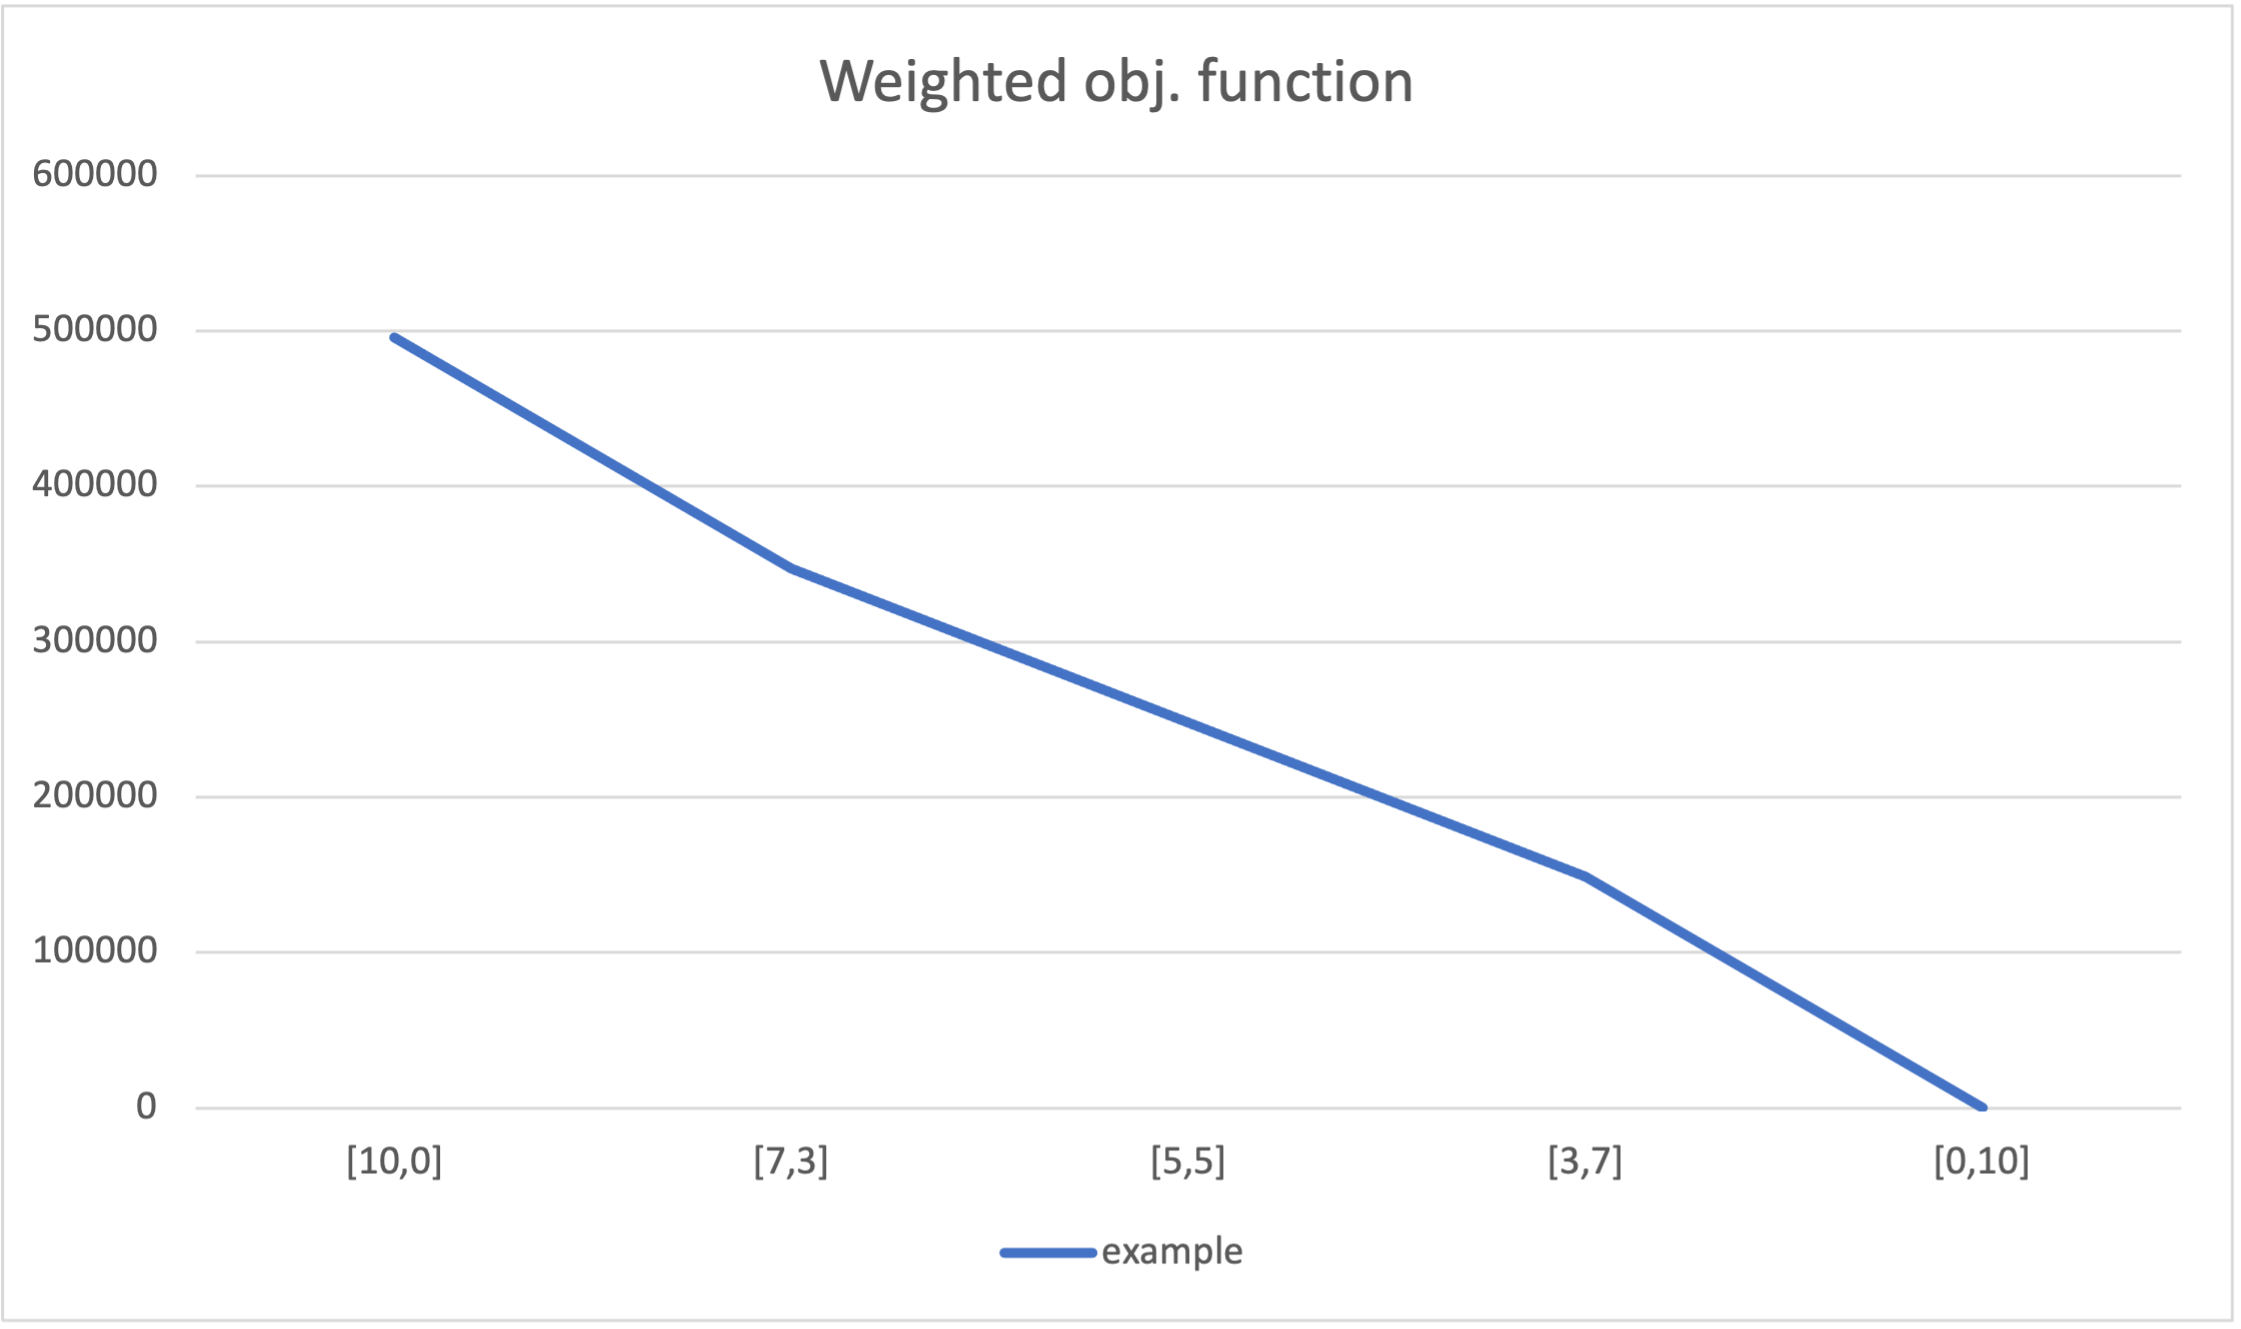
\includegraphics[height=0.25\textheight]{../graphs/example-wobjf.png}
    \caption{Weighted objective functions graph for example.}
\end{figure}

\begin{figure}[H]
    \centering
    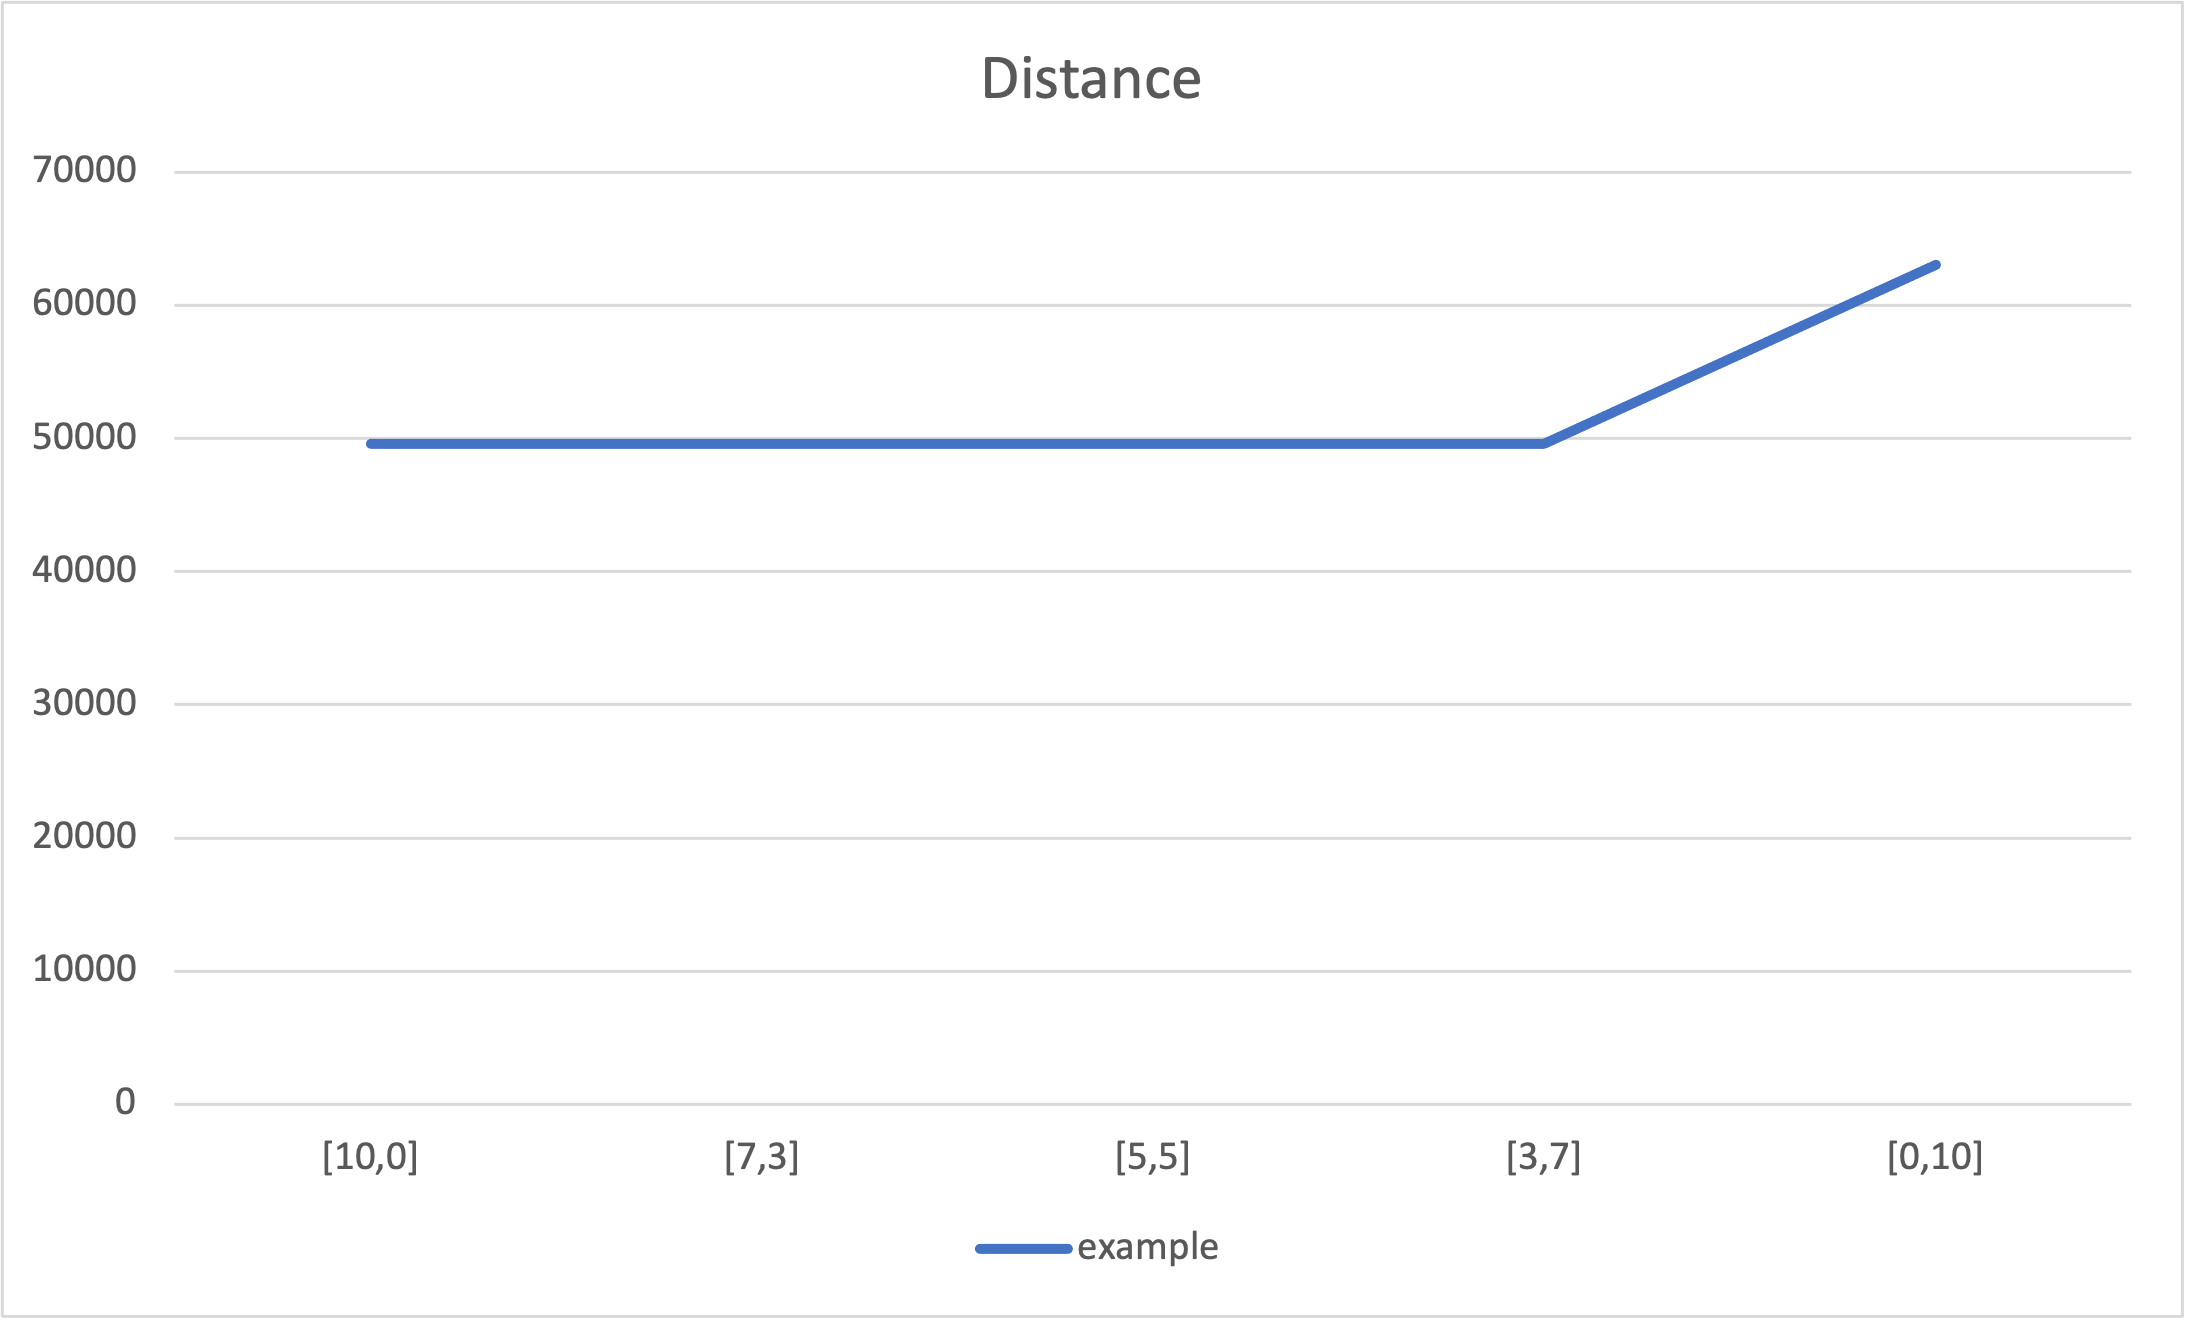
\includegraphics[height=0.25\textheight]{../graphs/example-distance.png}
    \caption{Distances graph for example.}
\end{figure}

\begin{figure}[H]
    \centering
    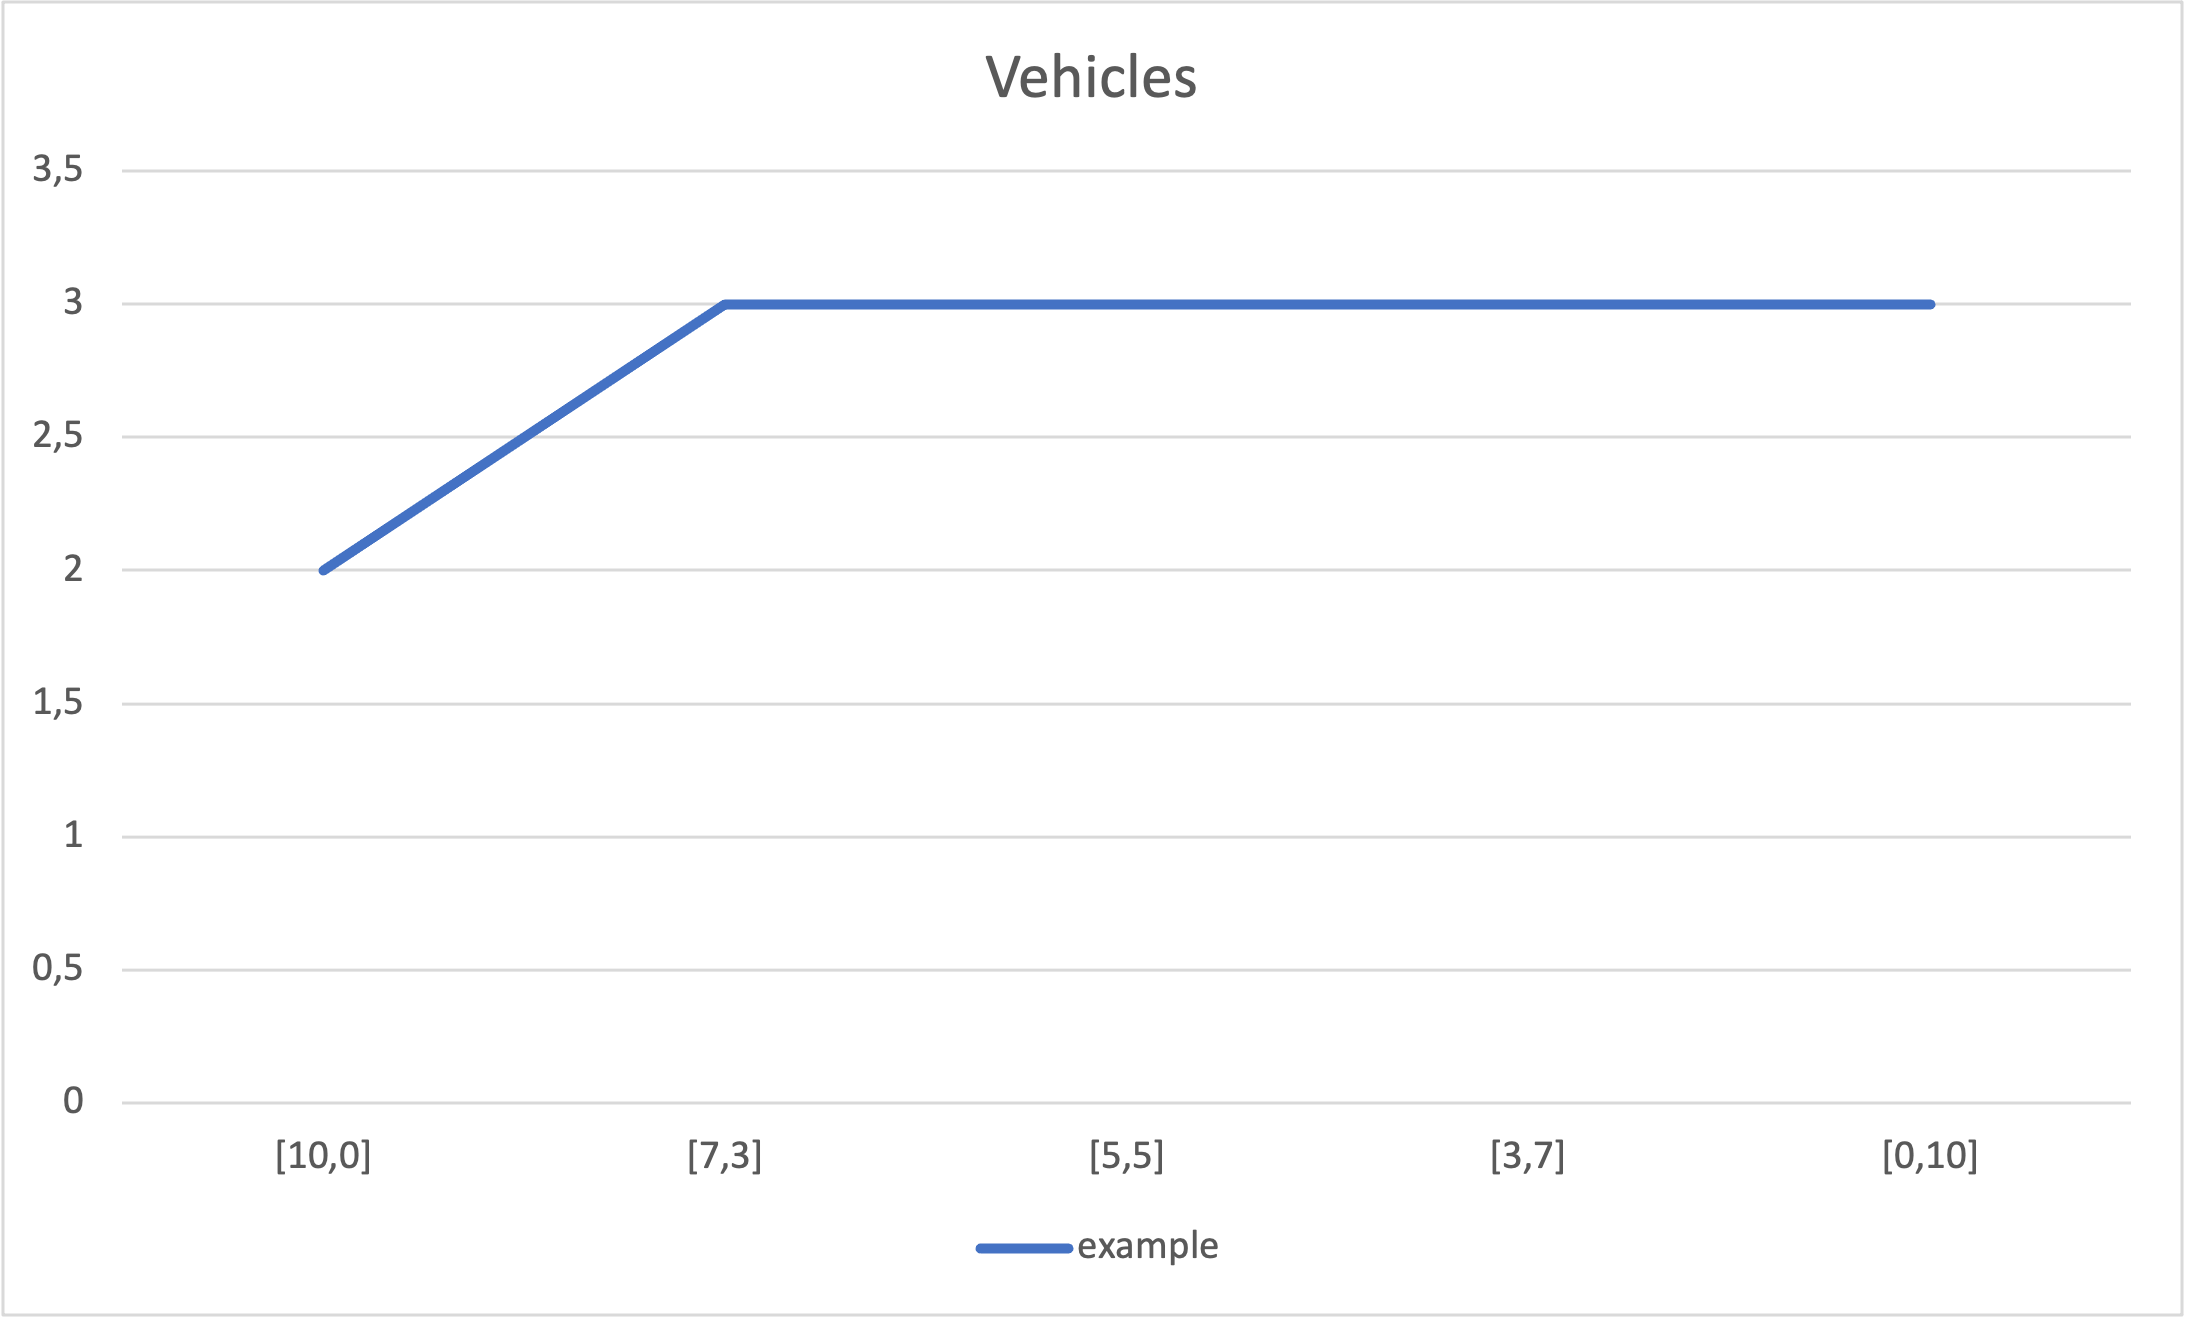
\includegraphics[height=0.25\textheight]{../graphs/example-vehicles.png}
    \caption{Vehicles used graph for example.}
\end{figure}

\newpage